\begin{flushleft}
\fontsize{12pt}{12pt} \timesbd{Introduction}\\
\end{flushleft}

%介紹論文的範圍和目標並說明問題
由於機器學習的訓練需要透過長時間的訓練,測試合適的機器學習算法和參數需要長時間的測試與訓練才能得到適用的演算法,若以實體的機電系統進行訓練需要投入大量的金錢與時間成本,採取虛擬訓練的方式:在相同時間下可以訓練的次數較多實體環境中多,改善訓練時間冗長和組裝實體系統的成本。測試在2D環境中的演算法在3D環境下的可行性並評估演算法若套用到實體系統可行性。\\

相關文獻\\

%描述方法
透過OpenAI Gym內建編譯的Pong 遊戲環境當作2D的訓練環境,3D則是透過CoppeilaSim來模擬訓練機電系統的運作狀況,訓練演算法選用強化學習結合類神經網路的學習方式,其中使用score function gradient當作主要算法。\\

概述工作的主要結果\\

%本文目的是將相同的訓練算法能在2D環境上進行訓練和使用,將相同演算法套用到3D模擬環境進行訓練與使用,以驗證算法若將既有機電系統簡化成2D所測試的算法套用到3D模擬環境的可行性。將實體冰球機的機電系統簡化後導入CoppeliaSim模擬環境透過Remote API控制環境中的冰球機移動,OpenCV來處理影像提供強化學習訓練和訓練後實際控制的輸入,強化學習訓練利用OpenAI Gym的Pong Game測試適合的訓練參數,再將算法套用到CoppeliaSim的場景中進行訓練。\\
%近年來硬體技術、軟體、自動求導等技術快速發展起來,再次帶起機器學習的發展,促使機器學習與各領域結合的應用越來越廣泛,在機電系統採用強化學習是為了讓機電系統的控制達到最佳化。本研究利用強化學習優化冰球機的對打系統,並測試相同演算法運用在2D與3D模擬環境可行性。\\
%本研究分成兩大部分,第一部分簡化冰球機並運用OpenAI Gym的Atari Pong-v0測試較合適的訓練參數,在2D環境中進行強化學習的對打訓練。第二部分獎實體系統簡化後導入CoppeliaSim模擬環境導入測試完成的訓練參數進行虛擬訓練,進行算法導入到實體機前的測試。\\

\begin{figure}[hbt!]	
	\centering
	\begin{subfigure}[]{placeholder}
		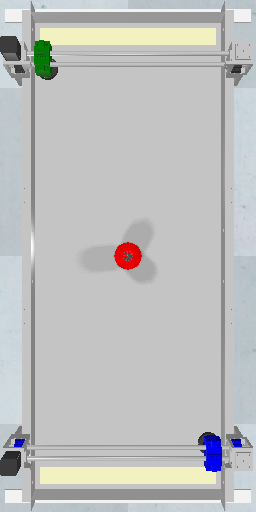
\includegraphics[width=4cm]{origin}
		\caption{Caption 1}\label{fig:1a}		
	\end{subfigure}
	\begin{subfigure}[]{placeholder}
		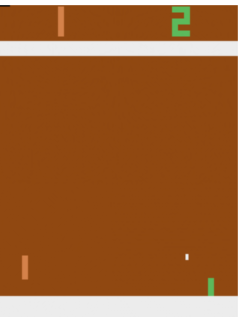
\includegraphics[width=4cm]{pong_gym}
		\caption{Caption 2}\label{fig:1b}
	\end{subfigure}
	\caption{Main figure caption}\label{fig:1}
\end{figure}
\newpage